\documentclass[12pt]{article}

\usepackage{setspace}
\usepackage{minted}
\usepackage{fancyvrb}
\usepackage{listings}
\usepackage{graphicx}

\usepackage[margin=0.75in]{geometry}
\pagestyle{empty}

\def \name       {Enrique Gavidia}
\def \coursenum  {CSC 415.01}
\def \coursename {Operating Systems Principles}
\def \instructor {Prof. Murphy}
\def \semester   {Spring 2012}
\def \assignment {Homework \# 7}
\def \duedate    {May 9, 2012}

\newcommand {\mytilde} {$\sim$}
\newcommand {\comment}[1] {\textcolor{red}{#1}}
\newcommand {\filename}[1] {\flushleft \textbf{#1}}
\newcommand {\append}[2] {\section*{Appendix #1} \textsl{\large #2}}

\newcommand {\makecover} {
  \begin{titlepage}
    \begin{center}
      \LARGE{\coursenum, \semester \\ \coursename}\\
      \Large{\instructor}\\
      \vfill
      \textbf{\Huge \assignment}\\
      \vfill
      \Large{\name}\\
      \large{\duedate}
    \end{center}
  \end{titlepage}
}

\DefineVerbatimEnvironment {shelloutput} {Verbatim} {fontsize=\scriptsize, numbers=left, frame=lines, commandchars=\%\{\}}

\newcommand {\includesource}[2] {\inputminted[linenos, fontsize=\scriptsize, frame=lines]{#1}{#2}}
\newcommand {\includeoutput}[1] {\VerbatimInput[fontsize=\scriptsize, numbers=left, frame=lines, commandchars=\%\{\}]{#1}}

\begin{document}

\makecover

%---{ Main Content }--------------------------------------------------------------------
\section*{Assignment Description}
Similar to our last project, this assignment was centered around the performance comparison of concurrent/parallel programs running 
on single and multi-core (in my case, Dual-core) unix/windows systems. Instead of searching however, we were to concurrently sort the 
different partitions of the array using the Insertion Sort algorithm, and retrieve the final sorted results dynamically using a 
\texttt{get\_next} function that incrementally retrieved the minimum of the smallest values from each of the sorted partitions. We were 
then to graph the results of running these programs on single and multi-core systems, again to visually compare the benefits of being able 
to run concurrent tasks in parallel. 

 
This code has been tested to work under \textsl{Windows}, \textsl{Gentoo Linux}, and \textsl{Mac OSX}.
The implementation for \textsl{Unix} is under \textbf{Appendix II}, and the \textsl{Windows} implementation is in \textbf{Appendix IV}. 
The \textsl{Pseudocode} outlining the design of both implementations is in \textbf{Appendix I}.
And the graphs for the outputs of the different systems are located under \textbf{Appendix VI}.


\section*{Design \& Implementation}
The design of these programs is rather simple, and fully outlined in the Pseudocode provided. The partitions are sorted just as their
respective threads are spawned, and then once all the partitions are sorted, the parent thread regains control and starts filling up
a new \texttt{sorted\_array} iteratively, using consecutive calls to the \texttt{get\_next} function. While filling up the \texttt{sorted\_array},
each value is passed through a custom assertion function to ensure that the values produced are in-fact sorted in non-decreasing order; if
the assertion check were to fail, the user is notified of the sorting error, and the program exits.  The \texttt{get\_next} functions similarly
to the one provided in the original assignment prompt, with the minor exception that mines also checks to make sure that the indices being
stored in the \texttt{minimums} array are valid for their respective partitions, so as to not accidentally step on the results of other 
partitions, or receive an out-of-bounds exception.


\section*{Results}
These programs were noticeably slower than the search-based counterparts we programmed in our last assignment, as expected; but it became apparent
that sorting algorithms (like Insertion Sort) lend themselves to better scalability with more concurrent/parallel systems. Concurrency mimics
the 'Divide and Conquer' method of problem solving, thus making each sub-problem smaller and quicker to solve. In the case of Insertion Sort,
this is due to the partitions requiring significantly less shifting of values every time an insertion is needed, than if the sort were performed
over the whole array.

Overall, the Windows and Unix implementations performed rather similarly, but there seemed to be a larger performance discrepancy between the unix machines, 
with the single-core one in particular showing clear signs of struggle handling multiple threads; while the windows version's single-core results were very 
consistent with its dual-core results.


\section*{Improvements}
Like for the last assignment, I would switch to using a linked-list instead of the array for the generated values to improve memory usage. Additionally, instead of storing and keeping
track of the entire sorted array at the end, I could switch to using a 2-item array for storing the \textsl{current} and \textsl{previous} values returned from the \texttt{get\_next} function,
which is all that should be needed to determine whether any of the values are not in sorted order; implementing this should cut down on memory usage a great deal.


%---{ Appendices }-----------------------------------------------------------------------
%\newpage

%----{ Unix }--------------------------------------------------------------------------

\append{I} {Pseudocode}
\begin{scriptsize}
\begin{verbatim}
int threads[];
int array[];
int array_size;
int sorted_array[];

semaphore sem;

sort_partition() {
    // sort array
    P(sem);
}

main() {

    // initialize random array...

    initialize_semaphore(s);

    for (thread in threads) {
        start_thread(thread, sort_partition)
    }

    for (thread in threads) {
        V(sem);
        end_thread(thread);
    }

    // check to make sure everything has been sorted right
    for (i = 0; i < array_size; i++) {
        sorted_array[i] = get_next();

        assert(sorted_array[i] >= sorted_array[i-1], "ERROR: Array was not sorted right");
    }
}
\end{verbatim}
\end{scriptsize}


\append{II} {Unix Source Code}
\includesource{c}{unix_sort.c}

\append{III} {Unix Output}
\filename{Single-core}
\includeoutput{output/unix_singlecore.txt}

\filename{Multi-core}
\includeoutput{output/unix_multicore.txt}

%----{ Windows }--------------------------------------------------------------------------
\append{IV} {Windows Source Code}
\includesource{c}{win_sort.c}

\append{V} {Windows Output}
\filename{Single-core}
\includeoutput{output/win_singlecore.txt}

\filename{Multi-core}
\includeoutput{output/win_multicore.txt}

\append{VI} {Graphs}
% Time (Y) vs # of Threads (x)


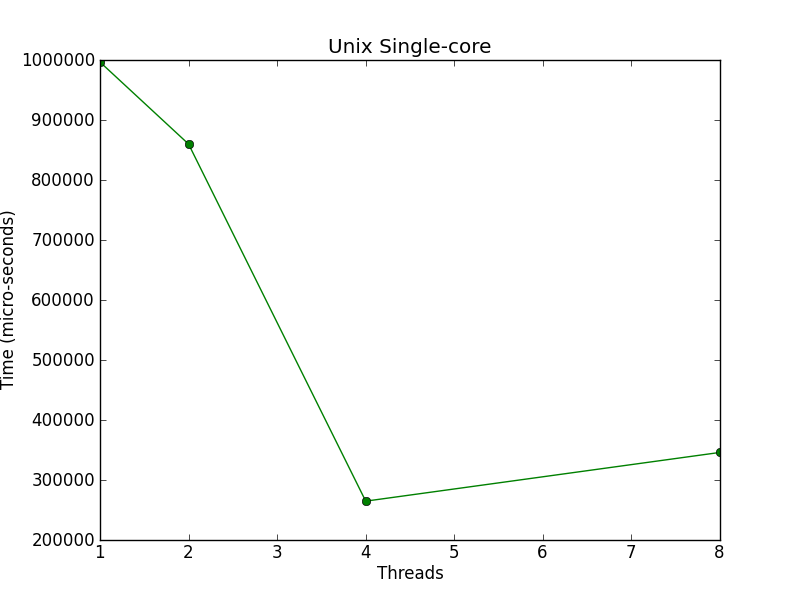
\includegraphics[scale=0.4]{output/graphs/unix_singlecore.png} 
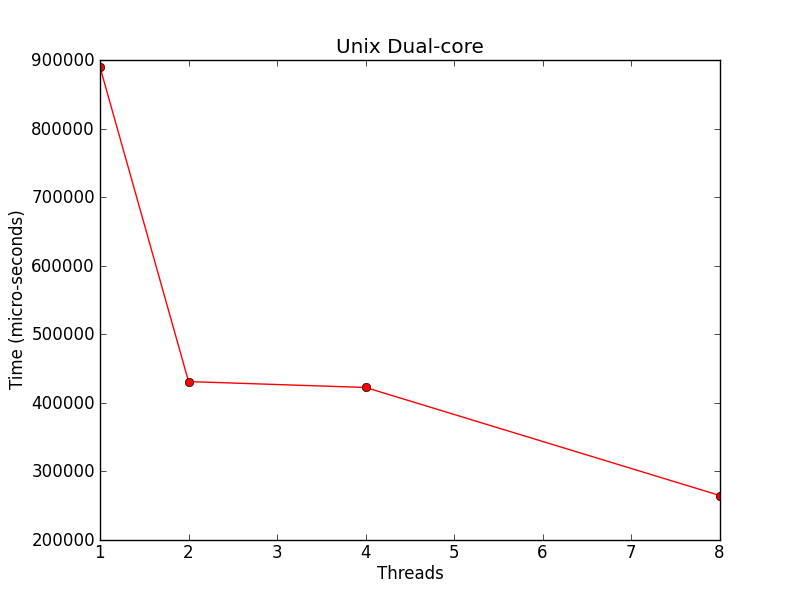
\includegraphics[scale=0.4]{output/graphs/unix_multicore.png}
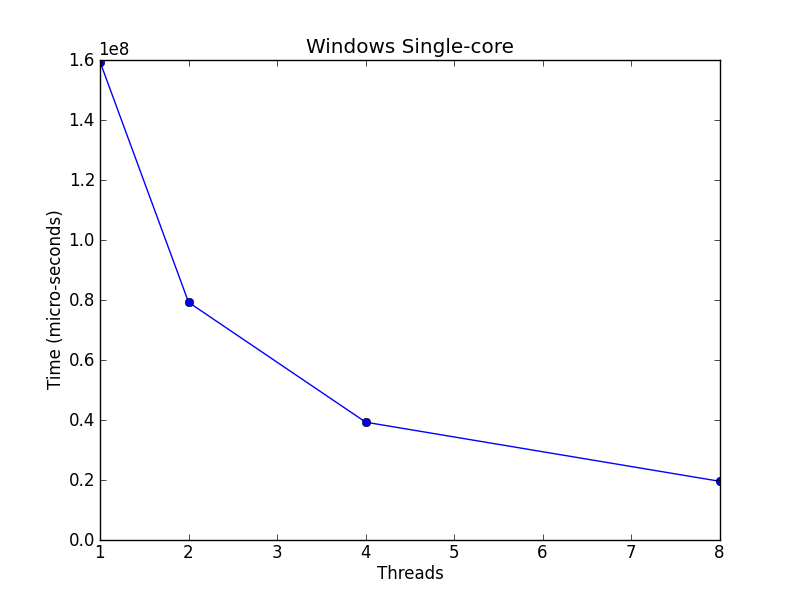
\includegraphics[scale=0.4]{output/graphs/win_singlecore.png} 
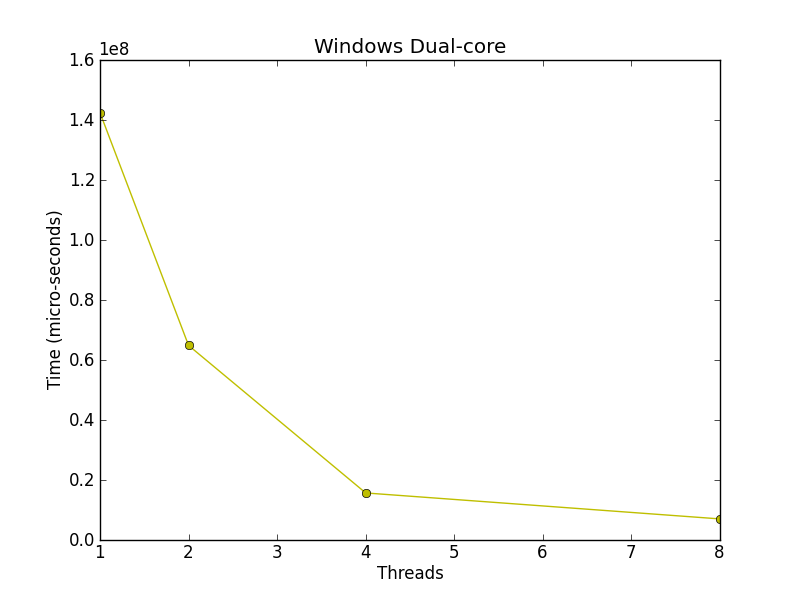
\includegraphics[scale=0.4]{output/graphs/win_multicore.png}


\end{document}
